\chapter{Tableur}  

Un tableur est un logiciel qui permet de faire des calculs à partir de tableaux contenant des nombres (les \emph{données}). Un tableur permet également de représenter ces données sous forme de graphiques qui en facilitent généralement la lecture.




%\phantom{rien}
{\footnotesize
\section*{Synoptique}

\begin{itemize}
\item Logiciel : \emph{Microsoft Excel}
\item Matières concernées : mathématiques, sciences physiques et géographie.
\item Compétences : 
        \begin{itemize}
        \item importer un fichier au format \texttt{CSV} ;
        \item référence variable et référence fixe ;
        \item trier des données ;
	\item fixer une ligne ou une colonne à l'affichage ;
	\item utiliser une condition pour définir le contenu d'une cellule ;
	\item naviguer dans une grande feuille de calcul.
        \end{itemize}
\item Cette fiche est à réaliser :
        \begin{itemize}
        \item avant les vacances d'octobre en mathématiques (séance 1) ;
        \item avant les vacances de printemps en sciences physiques (séance 2) ;
        \item avant la fin du semestre de cours en géographie (séance 3). 
        \end{itemize}
\end{itemize}
}



%\section*{Les années précédentes, vous avez appris...}

\vspace{12pt}

Les compétences listées ci-dessous ont été vues en classes de 6\up{e} et de 5\up{e}. Vous en aurez à nouveau besoin pour les activités de cette année. Si nécessaire, reportez-vous aux \emph{Fiches MITIC} des années précédentes pour revoir comment :  

\begin{itemize}
\item insérer une formule dans une cellule (6\up{e}) ;
\item utiliser la recopie incrémentale (6\up{e}) ;
\item tracer un graphique (nuage de points) (6\up{e}) ;
\item exporter la feuille et le graphique obtenus (6\up{e}) ;
\item définir le format d'une cellule (5\up{e}) ;
\item insérer une courbe de tendance dans un graphique (5\up{e}) ;
\item mettre en page une feuille de calcul (5\up{e}) ;
\item réaliser un diagramme circulaire (5\up{e}) ;
\item exporter un graphique, un tableau (5\up{e}).
\end{itemize}









%
%
%  S  É  A  N  C  E     I
%
%

%\newpage

\section{Séance 1 : Moyennes avec coefficients}\label{ficheTableur4e1}

\subsection{Pour préparer l'activité...}

\vspace{10pt}

Voici une vidéo pour apprendre à insérer un graphique avec \texttt{Excel}. Pensez à la regarder avant de commencer l'activité de la séance :

\begin{center}
\qrcode[hyperlink, height=0.9in]{https://web.microsoftstream.com/video/f327bedd-1400-47b8-afdc-905453577d47}
\end{center}

\vspace{12pt}

\subsection{Pour bien démarrer...}

\vspace{10pt}

Dès que vous avez ouvert un nouveau document dans \emph{Excel}, sauvegardez-le au format \texttt{Nom-seance1.xlsx} : dans le menu \texttt{Fichier}, choisir \texttt{Enregistrer sous}. Pendant que vous travaillez, pensez à sauvegarder régulièrement votre travail (raccourci clavier \texttt{Cmd + s}) si vous êtes sur l'application \emph{Excel}.

\uneimageici{./images/generales/clavierCmdS}{.4\textwidth}

Si vous êtes sur \emph{office.com}, vous n'avez besoin que d'enregistrer votre travail une première fois, les modifications étant automatiquement sauvegardées pendant que vous travaillez.

%\vspace{10pt}

\subsection{Sujet de l'activité...}

\vspace{10pt}

\boiteEnonceLarge{%
Le but de cette séance est de faire le calcul de la moyenne des élèves de 4\up{e} d'un établissement et de donner des informations par classe sur les résultats.
}
\vfill
\phantom{rien}
\boiteEnonceLarge{
À partir du fichier \texttt{ListeEleves\&Notes.xlsx} fourni par votre enseignant sur \emph{Teams}, il faut :
\begin{itemize}
\item figer les cellules pour que la première ligne soit toujours apparente;
\item trier les données pour trouver le meilleur élève de l'établissement, toutes classes confondues. Copier et coller son nom et sa moyenne dans les cellules \texttt{N3} et \texttt{O3};
\item calculer dans la cellule \texttt{I3} la moyenne de la première élève de la liste en tenant compte des coefficients qui se trouvent dans les cellules \texttt{E2} à \texttt{H2}.
\item tirer (recopie incrémentale) la formule trouvée pour obtenir la moyenne de tous les élèves (attention aux références variables);
\item dans la cellule \texttt{J3}, entrer la formule qui indique si l'élève est promu(e) ou redouble (condition sur la moyenne annuelle qui vient d'être calculée dans la colonne \texttt{I} puis tirer cette formule pour tous les élèves) ;
\item dans la cellule \texttt{K3}, écrire le texte «\,Nombre d'élèves promus :\,» et dans la cellule \texttt{L3}, entrer la formule qui calcule ce nombre automatiquement;
\item entrer le texte «\,nb. de redoublants :\,» dans la cellule \texttt{K4} puis tirer la formule entrée en \texttt{L3} dans la cellule \texttt{L4} (attention aux références variables) puis la modifier pour obtenir le nombre de redoublants;
\item trier les données par classe puis par moyenne pour donner le meilleur élève de chacune des classes (copier et coller le nom de l'élève et sa moyenne générale dans les cellules \texttt{N5} à \texttt{O12};
\item trier les élèves par classe puis calculer la moyenne de chacune des classes en utilisant la fonction \texttt{SOMME} pour calculer la somme des notes et \texttt{NB.SI} pour calculer le nombre d'élèves de la classe.
\end{itemize}
\vspace{10pt}
Une fois la mise en forme terminée, enregistrer le document au format XSLX en le nommant à partir de votre nom : \texttt{Nom-seance1.xlsx} puis rendre ce fichier sur \emph{Teams} à l'endroit indiqué par votre enseignant (si nécessaire, se reporter à la fiche méthode \emph{Remettre un devoir sur Teams}, page \pageref{TeamsRemettreDevoir}).
} % fin énoncé

\textbf{Pour obtenir de l'aide, rendez-vous à la page \pageref{AideTableur03}}

\subsection{Pour aller plus loin...}

Vous avez appris à utiliser trois fonctions du tableur : \texttt{SI}, \texttt{NB.SI} et \texttt{SOMME}. Mais il en existe beaucoup d'autres qui permettent d'automatiser de très nombreux calculs. Pour les découvrir et découvrir comment les utiliser, vous pouvez utiliser le \texttt{Concepteur de formules}. Pour y accéder, cliquez sur l'onglet \texttt{Insertion} \circled{1} puis sur le symbole de fonction f(x) à gauche \circled{2}:
\uneimageici{./images/tableur03/IconeFonction_OExcel_crop}{.4\textwidth}

\begin{itemize}
\item pour une meilleure lisibilité, utiliser la fonction \texttt{ARRONDI.AU.MULTIPLE} et afficher les moyennes arrondies au centième;
\item calculer la moyenne d'une classe en triant les données par \texttt{classe} puis en utilisant la fonction \texttt{MOYENNE} (déjà vue en 6\up{e}) ; tirer la formule trouvée dans les 7 cellules adjacentes pour obtenir les moyennes des 7 autres classes (attention aux références variables);
\item calculer la moyenne par classe sans avoir besoin de trier les données en utilisant les fonctions \texttt{NB.SI} et \texttt{SOMME.SI}.
\end{itemize}

\vfill

%\cadre{Pensez à sauver régulièrement votre travail en appuyant sur \texttt{Cmd + S} ou à partir du menu \texttt{Fichier} en choisissant \texttt{Enregistrer}.

%\uneimageici{./images/generales/clavierCmdS}{.5\textwidth}
%}






%
%
%  S  É  A  N  C  E     II
%
%


\pagebreak

\section{Séance 2 : Traitement de données}\label{ficheTableur4e2}

\subsection{Pour préparer l'activité...}

\vspace{10pt}

Voici une vidéo pour apprendre à insérer un trier les éléments d'un tableau avec \texttt{Excel}. Pensez à la regarder avant de commencer l'activité de la séance :

\begin{center}
\qrcode[hyperlink, height=0.9in]{https://web.microsoftstream.com/video/4f665642-b12f-42d8-8fc3-ab2c6f5b72db}
\end{center}

\vspace{12pt}

\subsection{Pour bien démarrer...}

Dès que vous avez ouvert un nouveau document dans \emph{Excel}, sauvegardez-le au format \texttt{Nom-seance2.xlsx} : dans le menu \texttt{Fichier}, choisir \texttt{Enregistrer sous}. Pendant que vous travaillez, pensez à sauvegarder régulièrement votre travail (raccourci clavier \texttt{Cmd + s}) si vous êtes sur l'application \emph{Excel}.

\uneimageici{./images/generales/clavierCmdS}{.4\textwidth}

Si vous êtes sur \emph{office.com}, vous n'avez besoin que d'enregistrer votre travail une première fois, les modifications étant automatiquement sauvegardées pendant que vous travaillez.

%\vspace{10pt}

\subsection{Sujet de l'activité...}

\vspace{10pt}


\boiteEnonceLarge{%
Le but de cette séance est de réaliser le traitement de données brutes fournies par la centrale d'acquisition ExAO de l'école. Les données collectées par ExAO sont exportées au format \texttt{CSV} (dans le logiciel \emph{Latis}, menu \texttt{Fichier}, choisir \texttt{Exportation} puis choisir le format de fichier \texttt{CSV}). 

\vspace{6pt}

Le fichier \texttt{CSV} est alors importé dans \emph{Excel} où les données sont traitées selon les consignes données par votre enseignant.

\vspace{6pt}

Une fois votre travail terminé, exporter votre graphique au format PNG en le nommant à partir de votre nom : \texttt{Nom-seance2.png} puis rendre ce fichier sur \emph{Teams} à l'endroit indiqué par votre enseignant (si nécessaire, se reporter à la fiche méthode \emph{Remettre un devoir sur Teams}, page \pageref{TeamsRemettreDevoir}).
}% fin énoncé



%\cadre{Pensez à sauver régulièrement votre travail en appuyant sur \texttt{Cmd + S} ou à partir du menu \texttt{Fichier} en choisissant \texttt{Enregistrer}.

%\uneimageici{./images/generales/clavierCmdS}{.5\textwidth}
%}

\textbf{Pour obtenir de l'aide, rendez-vous à la page \pageref{AideTableur03}}

\subsection{Pour aller plus loin...}

Chercher sur Internet ce qui caractérise un format CSV. Trouver un autre type très utilisé de structures de données.

\vfill
%
%
%  S  É  A  N  C  E     III
%
%



\pagebreak

\section{Séance 3 : Ressources en eau (géographie)}\label{ficheTableur4e3}

\subsection{Pour préparer l'activité...}

\vspace{10pt}

Voici une vidéo pour apprendre à insérer une condition pour l'affichage d'une cellule avec \texttt{Excel}. Pensez à la regarder avant de commencer l'activité de la séance :

\begin{center}
\qrcode[hyperlink, height=0.9in]{https://web.microsoftstream.com/video/d1e76f1b-4791-48ca-bd09-dbe319c2de29}
\end{center}

\vspace{12pt}

\subsection{Pour bien démarrer...}

\vspace{10pt}

Récupérer sur \emph{Teams} le fichier nommé \texttt{Geographie\_Eau\_Tableau.csv}, l'ouvrir avec \emph{Excel} et l'enregistrer au format XLSX (\texttt{Nom-seance3.xlsx}). Dans ce fichier, au départ, les pays sont classés par ordre alphabétique.

Dès que vous avez ouvert un nouveau document dans \emph{Excel}, sauvegardez-le au format \texttt{Nom-seance3.xlsx} : dans le menu \texttt{Fichier}, choisir \texttt{Enregistrer sous}. Pendant que vous travaillez, pensez à sauvegarder régulièrement votre travail (raccourci clavier \texttt{Cmd + s}) si vous êtes sur l'application \emph{Excel}.

\uneimageici{./images/generales/clavierCmdS}{.4\textwidth}

\subsection{Sujet de l'activité...}

\vspace{10pt}

\boiteEnonceLarge{%
Le but de cette séance est de retrouver et calculer des données dans un fichier au format \texttt{CSV} pour étudier les ressources en eau douce sur la planète.}
\vfill
\phantom{rien}
\boiteEnonceLarge{Pour cela :
\begin{itemize}
\item importer un fichier au format \texttt{CSV} dans \emph{Excel} ;
\item utiliser le tri de données pour faire apparaître le classement des pays en fonction de différents critères ;
\item déterminer à quel groupe les pays appartiennent en fonction de leurs ressources en eau en utilisant la fonction \texttt{SI};
\item calculer le nombre de pays appartenant à différents groupes en fonction de leurs ressources en eau, en utilisant la fonction \texttt{NB.SI};
\item insérer un diagramme circulaire représentant les ressources en eau des différents groupes.
\end{itemize}
\vspace{10pt}
Une fois la mise en forme terminée, exporter le document au format XLSX en le nommant à partir de votre nom : \texttt{Nom-seance3.xlsx} puis rendre ce fichier sur \emph{Teams} à l'endroit indiqué par votre enseignant (si nécessaire, se reporter à la fiche méthode \emph{Remettre un devoir sur Teams}, page \pageref{TeamsRemettreDevoir}).
}% fin énoncé


\subsection{Guide pour réaliser l'activité...}

%\subsection{Ressources en eau des différents pays}

\subsubsection{Ressources en eau par habitants}

Pour calculer les ressources en eau (nombre de m\up{3} par habitant\footnote{Un mètre-cube (m\up{3}) correspond à 1000\,litres}), entrer la formule permettant de faire le calcul pour le premier pays dans la cellule \texttt{G2} puis faire une recopie incrémentale de cette formule pour tous les pays.

\emph{Remarque :} la colonne des ressources en eau donne des valeurs en milliards de m\up{3}. Pour calculer les ressources en eau par habitant en \texttt{m\up{3} par habitant}, il faut multiplier le résultat par $10\up{9}$. Pour cela, on entre dans la cellule la formule suivante : \texttt{=(E2/F2)*10}\texttt{\^}\texttt{9}.

Trier ensuite les pays en fonction de la ressource en eau par habitant. Indiquer les 5 pays les plus «\,riches\,» en eau et les 5 pays les moins bien dotés par rapport à leur population en faisant un copier/coller de ces pays dans les cellules \texttt{K2} à \texttt{K6} et \texttt{K8} à \texttt{K12}.

\subsubsection{Ressources en eau par km\up{2}}

Entrer la formule permettant de faire le calcul des ressources en eau (en m\up{3}) par km\up{2} dans la colonne \texttt{H}.

Indiquer les 5 pays les plus «\,riches\,» et les 5 pays les moins bien dotés par rapport à leur superficie en faisant un copier/coller de ces pays dans les cellules \texttt{M2} à \texttt{M6} et \texttt{M8} à \texttt{M12}.


\subsubsection{Ressources en eau totales}

Trier les données du fichier pour identifier les 9 pays qui ont le plus de réserve en eau. Dans une cellule de votre choix, calculer la ressource en eau totale pour tous les pays et dans une autre cellule, la ressource en eau de ces 9 pays. Dans une troisième cellule, calculer le pourcentage d'eau possédée par ces pays (que vous pourrez comparer avec la valeur annoncée dans le document utilisé dans la partie \emph{Pour aller plus loin...}). Attention, pour les calculs des pourcentages, il faudra utiliser une référence fixe (se reporter au \S\ \vref{Calc3reference}).

\subsubsection{Ressources en eau, classement des pays en trois groupes}

Réaliser, dans la colonne \texttt{I}, les classement des pays en fonction du critère suivant : les pays qui disposent de moins de 1000 m\up{3} d'eau par habitant et par an sont classés dans le groupe des pays \texttt{pauvres en eau}. Les pays ayant entre 1000 et 8000 m\up{3} sont classés dans les pays \texttt{Moyennement dotés}. Enfin, les pays ayant plus de 8000 m\up{3} d'eau par habitant et par an sont classés dans le groupe des pays $\texttt{Riches en eau}$.
\begin{enumerate}
\item Dans la cellule \texttt{I2}, entrer la condition. Comme il y a trois cas possibles, les trois paramètres de la fonction \texttt{SI} sont les suivants :
  \begin{itemize}
    \item le premier paramètre est la première condition : \texttt{G2 < 1000} ;
    \item le deuxième paramètre est la valeur si la première condition est vraie : \texttt{"Pauvre en eau"};
    \item le dernier paramètre est la valeur si la première condition est fausse. Ce paramètre va à nouveau être une condition \texttt{SI} qui contient trois paramètres :
\begin{itemize}
 \item le premier paramètre est la deuxième condition : \texttt{G2 < 8000} ;
 \item le deuxième paramètre est la valeur si la deuxième condition est vraie : \texttt{"Moyennement doté"};
 \item le troisième paramètre est la valeur si la deuxième condition est fausse : \texttt{"Riche en eau"}.
\end{itemize}  
  \end{itemize}
\item Une fois la formule de la cellule entrée correctement, la tirer vers le bas pour avoir cette formule pour tous les pays.
\item Dans la cellule \texttt{I174}, calculer le nombre de pays \emph{«\,Pauvre en eau\,»} en utilisant la fonction \texttt{NB.SI}. Le premier paramètre à entrer est la liste des cellules sur lesquelles on fait le test (\texttt{I2} à \texttt{I172}). Le deuxième est la condition pour compter la cellule : \texttt{"Pauvre en eau"}.
\item Modifier la formule entrée dans la cellule \texttt{I174} pour que la liste des cellules sur lesquelles est fait le test ne soit pas modifiée lors d'une recopie incrémentale vers le bas, puis faire une recopie incrémentale de la formule dans les cellules \texttt{I175} et \texttt{I176}. Dans ces deux dernières cellules, modifier la condition pour compter le nombre de pays \texttt{"Moyennement dotés"} et de pays \texttt{"Riche en eau"}.
\item Insérer un diagramme circulaire représentant la part des ressources en eau des trois catégories de pays créées.
\end{enumerate}




\subsection{Pour aller plus loin...}

Pour répondre à la problématique de l'eau, récupérer sur la classe \emph{Teams} de votre cours les fichiers nommés :
\begin{itemize}
\item \texttt{Tableur3\_Seance3\_Geographie\_Texte\_Eau.txt} et
\item \texttt{Tableur3\_Seance3\_Geographie\_Eau\_Image.jpg}
\end{itemize}

\vspace{6pt}

Mettre en forme le fichier texte pour obtenir un résultat qui comprend :
\begin{itemize}
\item le titre dans l'en-tête de la première page;
\item une note de bas de page sur le titre pour indiquer la source du document;
\item un sommaire automatique (donc l'utilisation de style de paragraphe pour les titres);
\item des puces en plusieurs endroits ;
\item une image avec adaptation du texte ;
\item la numérotation des pages dans le pied de page avec un champ.
\end{itemize}

%\begin{center}
%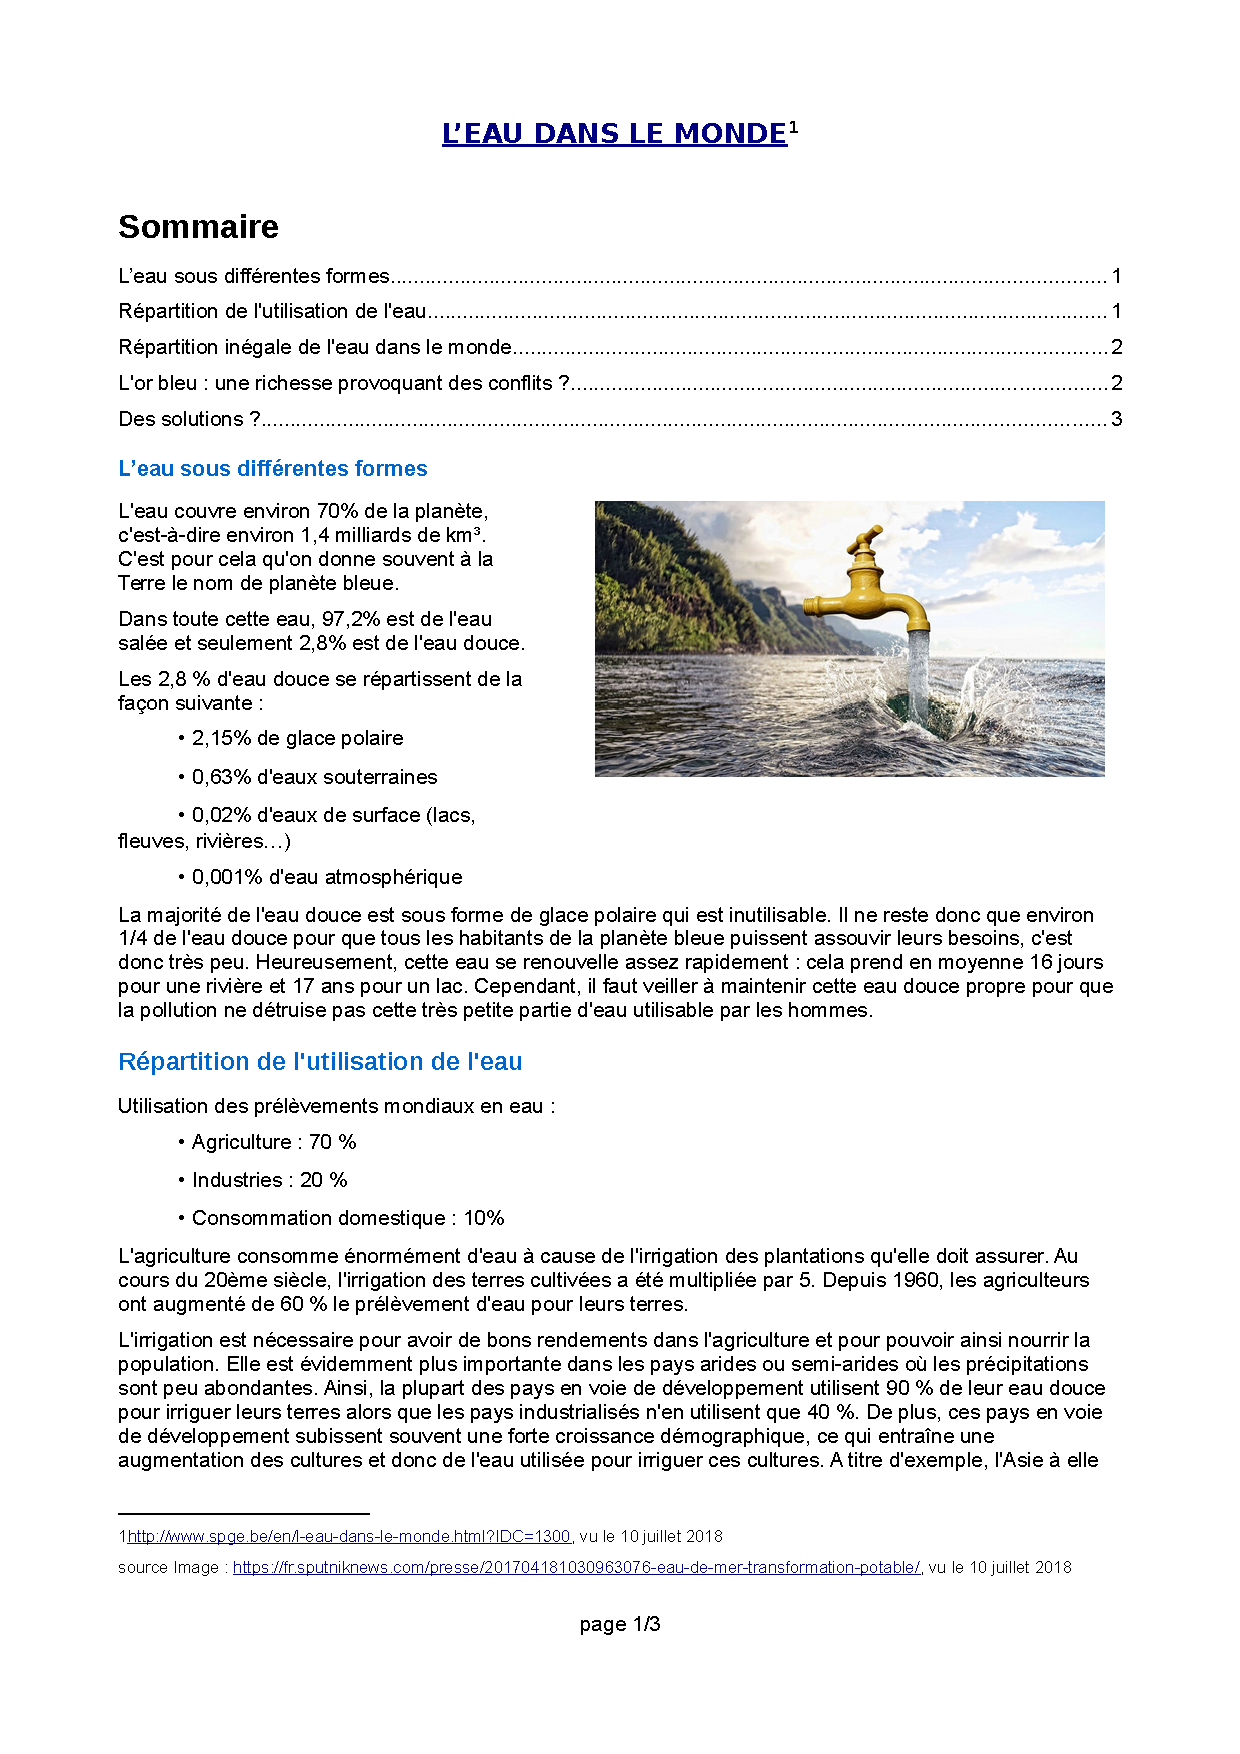
\includegraphics[width=0.65\textwidth]{./images/tableur03/Geographie_Texte_Eau_Page1}
%\end{center}

\vspace{-4em}



%\cadre{Pensez à sauver régulièrement votre travail en appuyant sur \texttt{Cmd + S} ou à partir du menu \texttt{Fichier} en choisissant \texttt{Enregistrer}.

%\uneimageici{./images/generales/clavierCmdS}{.25\textwidth}
%}



%
%
%  AIDES
%
%

\pagebreak

\section{Aide pour réaliser les activités}\label{AideTableur03}

Les nouveaux outils dont vous aurez besoin pour réaliser les séances sur le tableur sont décrits ci-dessous:
\begin{itemize}
	\item séparateur décimal, voir section \ref{Calc3sepDec} ;
	\item importer un fichier au format \texttt{CSV}, voir section \ref{Calc3fichierCSV}, page \pageref{Calc3fichierCSV} ;
	\item référence variable et référence fixe, voir section \ref{Calc3reference}, page \pageref{Calc3reference} ;
	\item trier des données, voir section \ref{Calc3tri}, page \pageref{Calc3tri} ;
	\item utiliser une condition pour définir le contenu d'une cellule, voir section \ref{Calc3Condition}, page \pageref{Calc3Condition} ;
	\item compter le nombre de cellules vérifiant une condition, voir section \ref{Calc3NBSI}, page \pageref{Calc3NBSI} ;
	\item additionner le contenu de plusieurs cellules, voir section \ref{Calc3Somme}, page \pageref{Calc3Somme} ;
	\item figer une ligne ou une colonne à l'affichage, voir section \ref{Calc3fixer}, page \pageref{Calc3fixer} ;
	\item naviguer dans une grande feuille de calcul, voir section \ref{Calc3navigue}, page \pageref{Calc3navigue}.
\end{itemize}




\subsection{Le séparateur décimal}\index{Calc!Séparateur décimal}\index{Séparateur décimal (Calc)}\index{Point ou virgule ? (Calc)}\index{Virgule ou point ? (Calc)}\index{Calc!Rechercher et remplacer}\index{Rechercher et remplacer (Calc)}\label{Calc3sepDec}

\subsubsection{Quel est votre séparateur décimal ?}


Le \emph{séparateur décimal} est le caractère utilisé pour écrire les nombres à virgule. En fonction de la langue du système d'exploitation de l'ordinateur on utilise pour les systèmes anglo-saxons, le point (ex. : $4.5$) ou pour les systèmes francophones, la virgule (ex. : $4,5$).

\vspace{6pt}

Dans \emph{Excel}, on peut déterminer si on utilise un point ou une virgule comme séparateur décimal. Pour cela, faire le test suivant : dans différentes cellules écrire un texte, un nombre entier et un nombre à virgule en utilisant une virgule puis un point. Les textes sont alignés à gauche et les nombres à droite. Dans les exemples ci-dessous, le séparateur décimal est donc la virgule pour l'image de gauche (le logiciel installé sur l'ordinateur) et le point pour l'image de droite (le logiciel accédé via office.com). Dans le premier cas, $3,14$ est reconnu comme un nombre et se retrouve aligné à droite, alors que $3.14$ se voit transformé en date (le 14 mars).

\deuximagesici{./images/tableur03/SeparateurDecimal_excel}{.5\textwidth}%  
{./images/tableur03/SeparateurDecimal_Oexcel_crop}{.5\textwidth}

Avant de faire une activité sur \emph{Excel}, pensez à vérifier si le séparateur décimal est le point ou la virgule chez vous. Vérifiez aussi, dans les exemples de ce chapitre, à vérifier si le séparateur correspond à celui de chez vous avant de recopier les valeurs. Si vous désirez avec le séparateur anglophone, le point, n'oubliez pas de remplacer les virgules par des points lorsque vous les copiez.

\subsubsection{Changer les virgules en points (ou inversement)}

Parfois il est nécessaire de changer toutes les virgules en points (ou inversement). C'est faisable sur la version logicielle d'\emph{Excel}. Pour cela, dans le menu \texttt{Édition}, choisir \texttt{Rechercher} puis \texttt{Remplacer...}

\uneimageici{./images/tableur03/changerVirgule1_excel_crop}{.7\textwidth}

Dans la boîte de dialogue qui s'ouvre (figure ci-dessous), indiquer le caractère à rechercher \circled{1} (ici la virgule) et le caractère de remplacement \circled{2} (ici le point). Pour terminer, cliquer sur \texttt{Remplacer tout} \circled{3} ce qui aura pour effet de remplacer en une fois tous les points du document.

\emph{Remarque : en cliquant sur \texttt{Remplacer}, une confirmation est demandée avant le remplacement de chaque point.}

\uneimageici{./images/tableur03/changerVirgule2_excel_crop}{.8\textwidth}


\subsection{Importer un fichier au format \texttt{CSV}}\index{Calc!Importer un fichier CSV}\index{Importer un fichier CSV (Calc)}\index{CSV : importer un fichier (Calc)}\label{Calc3fichierCSV}

Le format de fichier \texttt{CSV} (pour \emph{Comma-Separated Values}) est un format de fichier texte dans lequel des valeurs sont stockées séparées par une virgule. De nombreux logiciels permettent l'export de données au format \texttt{CSV} car c'est un format très simple et facilement lisible. Le logiciel qui pilote les platines ExAO, par exemple, permet l'export des données récoltées lors des expériences au format \texttt{CSV}.

Les fichiers \texttt{CSV} demandent une manipulation pour pouvoir être ouverts correctement sous \emph{Excel}, et la version en ligne ne permet pas de le faire.

\vspace{1em}

Pour ouvrir sous la version logicielle d'\emph{Excel} un fichier au format \texttt{CSV}, dans le menu \texttt{Fichier} \circled{1} choisir \texttt{Importer}. \circled{2} Dans la fenêtre qui s'ouvre, choisir \texttt{Fichier CSV} \circled{3}, puis \texttt{Importer}. \circled{4}

\deuximagesGPici{./images/tableur03/ImportCSV1_Excel_crop}{.8\textwidth}%
{./images/tableur03/ImportCSV2_Excel_crop}{\textwidth}

Dans la fenêtre suivante, choisir le fichier à importer et cliquer sur \texttt{Obtenir les données}. Une boîte de dialogue s'ouvre alors (figure ci-dessous). Normalement les options par défaut conviennent. 

\uneimageici{./images/tableur03/ImportCSV4_Excel_crop}{.6\textwidth}

La fenêtre suivante vous demande de sélectionner quels éléments séparent les valeurs. \circled{1} Dans cet exemple, il s'agit des virgules, il faut donc cocher la case correspondante. L'espace en bas donne un aperçu des données en tenant compte des séparateurs sélectionnés. \circled{2} Vérifiez bien que les colonnes sont celles que vous avez prévues d'exploiter, puis sélectionnez \texttt{Suivant >}. La dernière fenêtre vous permet de choisir le format des cellules que vous importez. Laissez \texttt{Général} coché et terminez l'importation en cliquant sur \texttt{Fin}, en bas à droite.

%\deuximagesGPici{./images/tableur03/ImportCSV3_Excel_crop}{.7\textwidth}%
%{./images/tableur03/ImportCSV4_Excel_crop}{\textwidth}

\uneimageici{./images/tableur03/ImportCSV3_Excel_crop}{.6\textwidth}



\textbf{Attention !} En fonction du paramétrage de votre système, il faut parfois transformer les points en virgules (ou inversement) pour que les valeurs importées soient reconnues comme des nombres (se reporter au paragraphe \vref{Calc3sepDec}).



\subsection{Référence variable et référence fixe}\index{Calc!Référence variable et référence fixe}\index{Calc!Tirer une formule en gardant une cellule fixe}\index{Référence variable et référence fixe (Calc)}\index{Tirer une formule en gardant une cellule fixe (Calc)}\label{Calc3reference} 

Lors d'une recopie incrémentale, c'est-à-dire lorsqu'on «\,tire\,» une formule comme montré en \circled{1} sur la figure ci-dessous à l'aide du coin de la cellule \circled{2}, la formule est adaptée ligne après ligne. On dit que la référence de la cellule est \emph{variable}. Pour comprendre il faut bien observer ce qu'il se passe sur les deux figures suivantes.

\uneimageici{./images/tableur03/RefFixeVariable1_Excel_crop}{.8\textwidth}

La formule à copier est \texttt{=(B3*B2+C3*C2+D3*D2)/SOMME(B2:D2)} : elle permet de calculer la moyenne de l'élève en tenant compte des coefficients contenus dans les cellules \texttt{B2} à \texttt{D2}.

Lorsqu'on va copier la formule, il faut donc que \texttt{B2}, \texttt{C2} et \texttt{D2} restent les références des cellules contenant les coefficients. Cependant, lors d'une recopie incrémentale si on ne prend pas des précautions on obtient la formule \texttt{(B4*\underline{B3}+C4*\underline{C3}+D4*\underline{D3})/(SOMME(\underline{B3}:\underline{D3}))}, ce qui est faux ! Les cellules contenant les coefficients ne sont plus les bonnes (figure ci-dessous).

\uneimageici{./images/tableur03/RefFixeVariable2_Excel_crop}{.8\textwidth}

Comment éviter ce problème lors de la recopie incrémentale ? Il faut simplement ajouter un signe \texttt{\$} devant le numéro des cellules des coefficients afin de préciser au tableur que lors de la recopie, ces numéros de cellules ne doivent pas être modifiés. La formule que l'on doit entrer en \texttt{E3} est donc la suivante :

\begin{center}\texttt{(B3*\underline{B\$2}+C3*\underline{C\$2}+D3*\underline{D\$2})/(SOMME(\underline{B\$2}:\underline{D\$2}))}\end{center}

On dit que la référence des cellules est \emph{fixe}. Elle ne sera plus modifiée par recopie (voir figure ci-dessous).

\uneimageici{./images/tableur03/RefFixeVariable3_Excel_crop}{.8\textwidth}

Maintenant lors de la recopie incrémentale les cellules contenant les coefficients ne sont pas modifiées (voir figure ci-dessous). Les moyennes sont maintenant justes !

\uneimageici{./images/tableur03/RefFixeVariable4_Excel_crop}{.8\textwidth}

Remarque : selon le même principe, il est possible de fixer la lettre de référence de la cellule. Ainsi, on peut écrire :

\begin{itemize}
	\item \texttt{\$B3} qui donnera par recopie incrémentale vers la droite \texttt{\$B3}, mais deviendra par recopie incrémentale vers le bas \texttt{\$B4} puis \texttt{\$B5}, etc.
	\item \texttt{\$B\$3} qui donnera par recopie incrémentale \texttt{\$B\$3} dans toutes les directions.
\end{itemize}

\subsection{Trier des données}\index{Calc!Trier des données}\index{Trier des données (Calc)}\label{Calc3tri} 

Dans un tableur, il est possible de trier les données contenues dans une feuille de calcul. Considérons par exemple une liste d'élèves, leur classe, leur moyenne annuelle et leur état de promotion. La première étape est de sélectionner les données que l'on souhaite trier, comme montré sur la figure ci-dessous \circled{1} (ici on sélectionne tout, donc le tri s'effectue sur toute la feuille, mais il est également possible de ne trier qu'une partie de la feuille). Dans le menu \texttt{Données} \circled{2} choisir alors \texttt{Tri personnalisé.} \circled{3}.

\uneimageici{./images/tableur03/TrierFiltrer1_OExcel_crop}{.7\textwidth}

Dans la boîte de dialogue qui s'ouvre, il faut choisir en fonction de quelle colonne on effectue le tri. Par exemple, comme montré au \circled{1} sur la figure à gauche ci-dessous, on peut demander de trier la colonne \texttt{Nom} (colonne qui contient les noms de famille des élèves). On peut également préciser \circled{2} si le tri doit être croissant (de A à Z) ou décroissant (de Z à A). En cliquant sur le bouton \texttt{OK}, la feuille de calcul est modifiée : les élèves sont maintenant triés par nom (figure à droite ci-dessous).

\deuximagesici{./images/tableur03/TrierFiltrer2a_OExcel_crop}{\textwidth}%
{./images/tableur03/TrierFiltrer2b_Excel_crop}{\textwidth}

Il est également possible de trier suivant plusieurs critères. Pour cela, dans la fenêtre dans laquelle on choisit le paramètre de tri, cliquer sur le \texttt{Ajouter} en haut à gauche. Une nouvelle ligne apparaît alors, qui permet de définir un nouveau critère de tri. Dans l'image ci-dessous à droite, on remarque que les élèves sont effectivement classés par classe, puis triès en fonction du nom de famille.

\deuximagesici{./images/tableur03/TrierFiltrer3a_OExcel_crop}{\textwidth}%
{./images/tableur03/TrierFiltrer3b_Excel_crop}{\textwidth}


% Finalement on laisse tomber les autofitres

% \subsection{Filtrer des données}\index{Calc!Filtrer des données}\index{Filtrer des données (Calc)}\label{Calc3filtre}

%\uneimageici{./images/tableur03/TrierFiltrer4}{.6\textwidth}

%\uneimageici{./images/tableur03/TrierFiltrer5}{.6\textwidth}

%\uneimageici{./images/tableur03/TrierFiltrer6}{.6\textwidth}

%\uneimageici{./images/tableur03/TrierFiltrer7}{.6\textwidth}






\subsection{Utiliser une condition pour définir le contenu d'une cellule}\index{Calc!Condition dans une cellule}\index{Condition dans une cellule (Calc)}\label{Calc3Condition}

On peut faire afficher dans une cellule un contenu qui dépend de la valeur d'une autre cellule. Par exemple, on va afficher pour chaque élève dans la colonne \texttt{promotion} le texte \emph{«\,promu(e)\,»} si sa moyenne est supérieure ou égale à 10, et \emph{«\,non promu(e)\,»} dans le cas contraire.

Il faut donc entrer une formule dans la première cellule de la colonne \texttt{promotion} : commencer par le signe \texttt{=} puis entrer \texttt{SI(}.


La formule que l'on doit entrer est la suivante : \textsl{si le contenu de la cellule} \texttt{D2} \textsl{est} $\geqslant 10$ \textsl{alors afficher «\,promu(e)\,» sinon afficher «\,non promu(e)\,»}. Dans \emph{Excel}, on utilise pour cela la fonction \texttt{SI} (en anglais : IF) qui doit être complétée tout d'abord avec le test à effectuer (ici \texttt{D5} $\geqslant 10$), puis avec la valeur que doit prendre la cellule si le test est vrai (ici «\,promu(e)\,») et enfin la valeur que doit prendre la cellule si le test est faux (ici «\,non promu(e)\,»).

\vspace{1em}

Dans le formalisme d'\emph{Excel}, cela s'écrit (ne pas oublier les virgules et les guillemets autour des textes !) :

\begin{center}
	\begin{tabular}{ccccccc}
		\texttt{=SI(} & \texttt{D2>=10} & , & \texttt{"promu(e)"} & , & \texttt{"non promu(e)"} & \texttt{)} \\ 
		Nom de & Test à  & & Valeur de la cellule & & Valeur de la cellule & \\
		la fonction & effectuer & &  si le test est vrai & & si le test est faux & \\  
	\end{tabular}
\end{center}

\uneimageici{./images/tableur03/condition3_OExcel_crop}{.6\textwidth}

Quand on appuie sur la touche \texttt{Entrée}, le résultat de la formule s'affiche. Sur la figure ci-dessous, on voit que Bruce, qui obtient 18,5 de moyenne annuelle, est promu. Il faut alors «\,tirer\,» la formule pour effectuer une recopie incrémentale. Pour cela, tirer la poignée comme montré sur la figure ci-dessous.

\uneimageici{./images/tableur03/condition4_Excel_crop}{.5\textwidth}

La figure ci-dessous présente le résultat.

\uneimageici{./images/tableur03/condition5_Excel_crop}{.5\textwidth}

\subsection{Compter le nombre de cellules vérifiant une condition}\index{Calc!Compter le nombre de cellules vérifiant une condition}\index{Compter le nombre de cellules vérifiant une condition (Calc)}\label{Calc3NBSI}

Pour calculer le nombre de cellules qui vérifient une condition donnée, par exemple pour calculer le nombre d'élèves promus, on se place dans la cellule dans laquelle on veut faire afficher le résultat (\texttt{G2} dans l'exemple ci-dessous). On utilise alors la fonction \texttt{NB.SI} qui utilise les paramètres suivants (ne pas oublier les virgules et les guillemets autour de la condition !) :


\begin{center}
	\begin{tabular}{cccccc}
		\texttt{=NB.SI(} & \texttt{D2:D6} & ; & \texttt{">=10"} &  &  \texttt{)} \\  
		Nom de & Plage de cellules  & & condition du test &  & \\
		la fonction & à tester (les moyennes) & &  entre guillemets : " " & & \\  
	\end{tabular}
\end{center}

\uneimageici{./images/tableur03/NBSI1_OExcel_crop}{.85\textwidth}


\emph{Remarque :} Après avoir écrit \texttt{=NB.SI(} et ouvert la parenthèse, on peut entrer à la main la plage de cellule concernées. On peut également, pour aller plus vite, sélectionner les cellules avec la souris ou en utilisant le clavier, puis continuer la formule en entrant le point-virgule et enfin la condition.



\subsection{Additionner le contenu de plusieurs cellules}\index{Calc!Somme de plusieurs cellules}\index{Somme de plusieurs cellules (Calc)}\label{Calc3Somme}

Pour faire la somme des valeurs de plusieurs cellules, on se place dans la cellule dans laquelle on veut afficher le résultat (\texttt{A5} dans l'exemple ci-dessous) et on écrit au clavier \texttt{=SOMME(} puis les cellules à ajouter (séparées par une virgule si on les entre une par une ou par \texttt{:} si on donne une plage de plusieurs cellules) avant de refermer la parenthèse, de la manière suivante :

\begin{center}
	\begin{tabular}{ccc}
		\texttt{=SOMME(} & \texttt{A1:A4} &   \texttt{)} \\  
		Nom de & Plage de cellules  & \\
		la fonction & à ajouter & \\  
	\end{tabular}
\end{center}

\uneimageici{./images/tableur03/FonctionSomme_Excel_crop}{.4\textwidth}

\subsection{Figer une ligne ou une colonne à l'affichage}\index{Calc!Fixer une ligne ou une colonne}\index{Fixer une ligne ou une colonne (Calc)}\label{Calc3fixer} 

Dans les grandes feuilles de calcul, il peut être utile de \emph{figer} une ligne ou une colonne, c'est-à-dire de faire en sorte qu'elle reste en permanence affichée même si on descend dans la feuille de calcul (c'est souvent la ligne contenant le titre des colonnes).

%\vspace{1em}

Pour figer une ligne, aller dans l'onglet \texttt{Affichage} \circled{1} puis cliquer sur \texttt{Figer les volets} \circled{2} et enfin sur \texttt{Figer la ligne supérieure} \circled{3}. Attention : il faut pour cela que la ligne en haut de l'affichage soit la ligne 1. Sinon, \emph{Excel} va figer une autre ligne!

\uneimageici{./images/tableur03/figerFenetre1_OExcel_crop}{.8\textwidth}

Le résultat est montré ci-dessous : la ligne 1 de la feuille de calcul est toujours affichée et elle est suivie de... la ligne 440 !

\uneimageici{./images/tableur03/figerFenetre2_Excel_crop}{.4\textwidth}

\emph{Remarque :} pour faire cesser la fixation d'une ligne, il suffit de cliquer sur \texttt{Libérer les volets}, situé également sous \texttt{Figer les volets}.


\subsection{Naviguer dans une grande feuille de calcul}\index{Calc!Naviguer dans une grande feuille}\index{Naviguer dans une grande feuille (Calc)}\index{Déplacements dans une grande feuille de calcul (Calc)}\label{Calc3navigue} 
Pour se déplacer rapidement dans les grandes feuilles de calculs, le plus simple est d'utiliser le clavier. Il permet également de sélectionner de grandes plages de valeurs.

La première étape est à chaque fois de se placer sur une cellule de la colonne ou de la ligne dans laquelle on veut se déplacer. On peut alors se déplacer très rapidement en appuyant sur les combinaisons de touches suivantes :

\begin{center}
	\begin{tabular}{ll}
		\textsl{Aller tout en bas d'une colonne} & 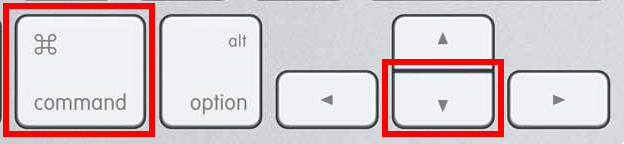
\includegraphics[width=4cm]{./images/tableur03/clavierCmDdown} \\     
		\textsl{Aller tout en haut d'une colonne} & 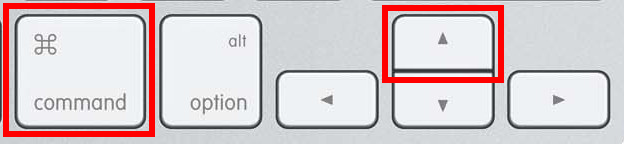
\includegraphics[width=4cm]{./images/tableur03/clavierCmDup} \\  
		\textsl{Aller à la fin d'une ligne} & 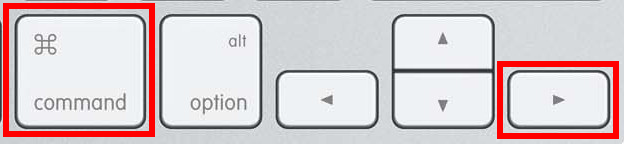
\includegraphics[width=4cm]{./images/tableur03/clavierCmDright} \\  
		\textsl{Aller au début d'une ligne} & 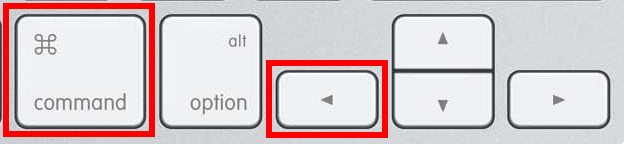
\includegraphics[width=4cm]{./images/tableur03/clavierCmDleft} \\  
	\end{tabular}
\end{center}

Si on utilise ces touches alors que le curseur se trouve sur une cellule vide, il se déplacera à la place vers la première cellule avec du contenu dans la direction indiquée.

Si de plus on souhaite sélectionner les cellules alors on utilise la touche \texttt{Shift}. Par exemple, pour sélectionner entièrement les nombres contenus dans une grande ligne, on se place sur la première valeur de la ligne puis on appuie sur la combinaison de touches :

\begin{center}
	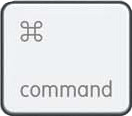
\includegraphics[scale=1.5]{./images/tableur03/clavierCmd}  + 
\includegraphics[scale=1.5]{./images/tableur03/clavierShift} + 
\includegraphics[scale=1.5]{./images/tableur03/clavierRight}
\end{center}